% REMEMBER: You must not plagiarise anything in your report. Be extremely careful.
\documentclass{l4proj}

    
%==============================================================================
% Put any additional packages here
% You can add any packages you want, as long as it does not alter
% the overall format (e.g. don't change the margins or the reference style).
%
\usepackage{pdfpages} % if you want to include a PDF for an ethics checklist, for example
%
%

\usepackage{tikz}
\usepackage{float}
\usepackage{enumitem}

\lstdefinelanguage{TML}{ 
    keywords={changeto, move, goto, if, switch, while, module, accept, reject, halt, alphabet},
    ndkeywords={left, right, tapehead, blank},
    sensitive=true,
    comment=[l]{//},
    morecomment=[s]{/*}{*/},
    morestring=[b]',
    morestring=[b]"
}

\newtheorem{theorem}{Theorem}

\begin{document}

%==============================================================================
%% METADATA
\title{Turing Machine Language} % change this to your title
\author{Pete Gautam}

\maketitle

%==============================================================================
%% ABSTRACT
\begin{abstract}
    % Every abstract follows a similar pattern. Motivate; set aims; describe work; explain results.
    % \vskip 0.5em
    % ``XYZ is bad. This project investigated ABC to determine if it was better. 
    % ABC used XXX and YYY to implement ZZZ. This is particularly interesting as XXX and YYY have
    % never been used together. It was found that  
    % ABC was 20\% better than XYZ, though it caused rabies in half of subjects.''
\end{abstract}

%==============================================================================
%% ACKNOWLEDGEMENTS
\chapter*{Acknowledgements}
% Enter any acknowledgements here. This is optional; you may leave this blank if you wish,
% or remove the entire chapter
%
% We give thanks to the Gods of LaTeX, who in their eternal graciousness, 
% have granted that this document may compile without errors or overfull hboxes.
%

%==============================================================================

% EDUCATION REUSE CONSENT FORM
% If you consent to your project being shown to future students for educational purposes
% then insert your name and the date below to  sign the education use form that appears in the front of the document. 
% You must explicitly give consent if you wish to do so.
% If you sign, your project may be included in the Hall of Fame if it scores particularly highly.
%
% Please note that you are under no obligation to sign 
% this declaration, but doing so would help future students.
%
\def\consentname {Pete Gautam} % your full name
\def\consentdate {27 September 2022} % the date you agree
%
\educationalconsent


%==============================================================================
\tableofcontents

%==============================================================================
%% Notes on formatting
%==============================================================================
% The first page, abstract and table of contents are numbered using Roman numerals and are not
% included in the page count. 
%
% From now on pages are numbered
% using Arabic numerals. Therefore, immediately after the first call to \chapter we need the call
% \pagenumbering{arabic} and this should be called once only in the document. 
%
%
% The first Chapter should then be on page 1. 

% PAGE LIMITS
% You are allowed 40 pages for a 40 credit project and 30 pages for a 
% 20 credit report. 
% This includes everything numbered in Arabic numerals (excluding front matter) up
% to but *excluding the appendices and bibliography*.
%
% FORMATTING
% You must not alter text size (it is currently 10pt) or alter margins or spacing.
% Do not alter the bibliography style. 
%
%==================================================================================================================================
%
% IMPORTANT
% The chapter headings and structure here are **suggestions**. You don't have to follow this model if
% it doesn't fit your project. Every project should have an introduction and conclusion,
% however.  If in doubt, your supervisor can give you specific guidance; their view takes precedence over
% the structure suggested here.
%
%==================================================================================================================================
\chapter{Introduction}

% reset page numbering. Don't remove this!
\pagenumbering{arabic} 

% \todo{Remove the guidance notes from your dissertation before submitting!}

% Why should the reader care about what are you doing and what are you actually doing?
% \section{Guidance}

% \textbf{Motivate} first, then state the general problem clearly. 

% \section{Writing guidance}
% \subsection{Who is the reader?}

% This is the key question for any writing. Your reader:

% \begin{itemize}
%     \item
%     is a trained computer scientist: \emph{don't explain basics}.
%     \item
%     has limited time: \emph{keep on topic}.
%     \item
%     has no idea why anyone would want to do this: \emph{motivate clearly}
%     \item
%     might not know \emph{anything} about your project in particular:
%     \emph{explain your project}.
%     \item
%     but might know precise details and check them: \emph{be precise and
%     strive for accuracy.}
%     \item
%     doesn't know or care about you: \emph{personal discussions are
%     irrelevant}.
% \end{itemize}

% Remember, you will be marked by your supervisor and one or more members
% of staff. You might also have your project read by a prize-awarding
% committee or possibly a future employer. Bear that in mind.

% \subsection{References and style guides}
% There are many style guides on good English writing. You don't need to
% read these, but they will improve how you write.

% \begin{itemize}
%     \item
%     \emph{How to write a great research paper} \cite{Pey17} (\textbf{recommended}, even though you aren't writing a research paper)
%     \item
%     \emph{How to Write with Style} \cite{Von80}. Short and easy to read. Available online.
%     \item
%     \emph{Style: The Basics of Clarity and Grace} \cite{Wil09} A very popular modern English style guide.
%     \item
%     \emph{Politics and the English Language} \cite{Orw68}  A famous essay on effective, clear writing in English.
%     \item
%     \emph{The Elements of Style} \cite{StrWhi07} Outdated, and American, but a classic.
%     \item
%     \emph{The Sense of Style} \cite{Pin15} Excellent, though quite in-depth.
% \end{itemize}

% \subsubsection{Citation styles}

% \begin{itemize}
% \item If you are referring to a reference as a noun, then cite it as: ``\citet{Orw68} discusses the role of language in political thought.''
% \item If you are referring implicitly to references, use: ``There are many good books on writing \citep{Orw68, Wil09, Pin15}.''
% \end{itemize}

% There is a complete guide on good citation practice by Peter Coxhead available here: \url{http://www.cs.bham.ac.uk/~pxc/refs/index.html}. 
% If you are unsure about how to cite online sources, please see \citet{UNSWWebsite}. 
% \footnote{Specifying an online resource like \url{https://developer.android.com/studio}
% in a footnote sometimes makes more sense than including it as a formal reference.}

% \subsection{Plagiarism warning}

% \begin{highlight_title}{WARNING}
    
%     If you include material from other sources without full and correct attribution, you are commiting plagiarism. The penalties for plagiarism are severe.
%     Quote any included text and cite it correctly. Cite all images, figures, etc. clearly in the caption of the figure.
% \end{highlight_title}

% \subsection{Quoting text}

% If you are quoting a long passage, use a \texttt{quote} environment:

% \begin{quote}
%      If you scribble your thoughts any which way, your readers will surely feel that you care nothing about them. They will mark you down as an egomaniac or a chowderhead -or, worse, they will stop reading you. The most damning revelation you can make about yourself is that you do not know what is interesting and what is not.
% \end{quote} \citep{Von80}

% If you are quoting inline, like Simon Peyton-Jones' following remark, use quotation marks ``Conveying the intuition is primary, not
% secondary'' \citep{Pey17}.


%==================================================================================================================================
\chapter{Background}
\section{Turing Machine}
\subsection{Introduction to Turing Machines}
A \emph{Turing Machine} (TM) is a collection $(Q, \Sigma, \delta, q_0)$, where:
\begin{itemize}
    \item $Q$ is a set of \emph{states}, including the \emph{accept state} $A$ and \emph{reject state} $R$;
    \item $\Sigma$ is the set of \emph{letters}, which does not include the \texttt{blank} symbol;
    \item $\delta \colon Q \setminus \{A, R\} \times \Sigma^+ \to Q \times \Sigma^+ \times \{\texttt{left}, \texttt{right}\}$, where $\Sigma^+ = \Sigma \cup \{\texttt{blank}\}$, is the \emph{transition function}; and
    \item $q_0 \in Q$ is the \emph{starting state}.
\end{itemize}
Although based on Turing's work on \cite{turing1936computable}, this definition, along with others in this section, have been adapted from \cite{hopcroft2001automata}.

\begin{figure}[htb]
    \centering
    \begin{subfigure}{0.45\textwidth}
        \centering
        \begin{tikzpicture}
            \node[state, accepting] (q0) at (0, 0) {$q_0$};
            \node[state] (q1) at (2.5, 0) {$q_1$};
            \node[state, fill=green, opacity=0.6] (A) at (5, -1) {$A$};
            \node[state, fill=red, opacity=0.6] (R) at (5, 1) {$R$};
    
            \draw[->] (q0) edge[loop above] node[text width=1.5cm, align=center] {$0 \to 0, R$ $1 \to 1, R$} (q0);
            \draw[->] (q0) -- node[above] {$\# \to \#, L$} (q1);
            \draw[->] (q1) -- node[below, rotate=-20] {$0 \to \#, L$} (A);
            \draw[->] (q1) -- node[above, rotate=20, text width=1.5cm, align=center] {$1 \to 1, L$ $\# \to \#, L$} (R);
        \end{tikzpicture}
        \caption{Full notation}
    \end{subfigure}
    \hfill
    \begin{subfigure}{0.45\textwidth}
        \centering
        \begin{tikzpicture}
            \node[state, accepting] (q0) at (0, 0) {$q_0$};
            \node[state] (q1) at (2.5, 0) {$q_1$};
            \node[state, fill=green, opacity=0.6] (A) at (5, -1) {$A$};
            \node[state, fill=red, opacity=0.6] (R) at (5, 1) {$R$};
    
            \draw[->] (q0) edge[loop above] node {$0|1, R$} (q0);
            \draw[->] (q0) -- node[above] {$\#, L$} (q1);
            \draw[->] (q1) -- node[below, rotate=-20] {$0 \to \#, L$} (A);
            \draw[->] (q1) -- node[above, rotate=20] {$1|\#, L$} (R);
        \end{tikzpicture}
        \caption{Shorthand notation}
    \end{subfigure}
    \caption{A FSM representation of a TM that accepts binary numbers divisible by 2.}
    \label{fig:tm_isDiv2}
\end{figure}

We can represent a TM as a finite state machine (FSM). This is a directed graph, with vertices as states and edges as transitions. An example is given in Figure \ref{fig:tm_isDiv2}. In this case, the alphabet $\Sigma = \{0, 1\}$. The blank symbol is denoted by $\#$. The initial state is denoted by $q_0$; the accept state $A$ and the reject state $R$. Every edge corresponds to an evaluation of the transition function $\delta$, e.g. $\delta(q_1, 0) = (A, \texttt{blank}, \texttt{left})$. 

The figure presents two ways of representing a FSM- subfigure (a) shows all the transitions, while subfigure (b) only shows the transitions where the tapehead value is getting changed. It also combines certain letters if they are not being changed. We will make use of the shorthand FSM representation from now.

\subsection{Executing a TM on a tape}
Let $\Sigma$ be an alphabet. A \emph{tape} $T$ on $\Sigma$ is a function $T\colon \mathbb{Z} \to \Sigma^+$. In particular, the tape has infinite entries in both directions. 

\begin{figure}[htb]
    \centering
    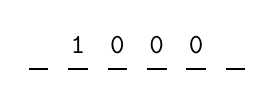
\begin{tikzpicture}
        \foreach \x[count=\i] in {, 1, 0, 0, 0, } {
            \draw[thick] (\i*0.5-0.25, 0) -- (\i*0.5, 0);
            \node at (\i*0.5-0.125, 0.3) {\texttt{\x}};
        }
    \end{tikzpicture}
    \caption{A TM tape on $\{0, 1\}$.}
    \label{fig:tape_example}
\end{figure}
We can represent a tape using a figure. For instance, let $\Sigma = \{0, 1\}$, and let $T$ be the tape on $\Sigma$ given below:
\[T(x) = \begin{cases}
    0 & x \in \{0, 2, 3\} \\
    1 & x \in \{1\} \\
    \texttt{blank} & \text{otherwise}.
\end{cases}\]
Then, Figure \ref{fig:tape_example} represents the tape $T$. We will assume that the first non-blank value is at index 0.

We can execute a TM on a tape. Let $M$ be a TM with alphabet $\Sigma$, and let $T$ be a tape on $\Sigma$. We execute $M$ on $T$ inductively, as follows:
\begin{itemize}
    \item At any point during execution, we maintain 3 objects:
    \begin{enumerate}
        \item a tape on $\Sigma$, 
        \item a (current) state in $M$ and 
        \item an index in the tape (called the \emph{tapehead index}). 
    \end{enumerate}
    
    \item At the start,
    \begin{enumerate}
        \item the tape is $T$; 
        \item the tapehead index is $0$; and
        \item the current state is the initial state $q_0$. 
    \end{enumerate}
    
    \item At some point during the execution, assume that we have the tape $S$, tapehead index $j$, with \emph{tapehead value} $T(j) = t$, and a non-terminating state $q$ (i.e. not $A$ or $R$). Denote $\delta(q, t) = (q', t', \texttt{dir})$. Then, 
    \begin{enumerate}
        \item the next state is $q'$;
        \item the next tape is $S'$, where
        \[S'(x) = \begin{cases}
            t' & x = i \\
            S(x) & \text{otherwise};
        \end{cases}\]
        and
        \item the next tapehead index is $j'$, where
        \[j' = \begin{cases}
            j+1 & \texttt{dir} = \texttt{right} \\
            j-1 & \texttt{dir} = \texttt{left}.
        \end{cases}\]
    \end{enumerate}
    If the state $q'$ is not a terminating state, then the execution continues with these 3 objects. Otherwise, execution is terminated with terminating state $q'$.
\end{itemize}

We illustrate this process with the TM in Figure \ref{fig:tm_isDiv2} with the tape in Figure \ref{fig:tape_example}:
\begin{itemize}
    \item Initially, 
    \begin{enumerate}
        \item the tape is the given tape;
        \item $q_0$ is the current state; and 
        \item the tapehead index is $0$, with value $1$.
    \end{enumerate}
    \item According to the FSM, we have $\delta(q_0, 1) = (q_0, 1, R)$. Hence,
    \begin{enumerate}
        \item the tape remains unchanged;
        \item $q_0$ is still the current state; and
        \item and the tapehead index becomes $1$, with value is \texttt{0}.
    \end{enumerate}
    \item The transition for \texttt{0} and \texttt{1} are the same with respect to $q_0$. This means that we keep moving to the right until we end up at a blank symbol. At that point, the following is the state of the tape:
    \begin{figure}[H]
        \centering
        \begin{tikzpicture}
            \foreach \x[count=\i] in {, 1, 0, 0, 0, } {
                \draw[thick] (\i*0.5-0.25, 0) -- (\i*0.5, 0);
                \node at (\i*0.5-0.125, 0.3) {\texttt{\x}};
            }
            \draw[->] (2.875, -0.5) -- (2.875, -0.1);
        \end{tikzpicture}
    \end{figure}
    The arrow points at the tapehead value. We are still at the state $q_0$, and the tape has not been altered.
    
    \item Now, since the tapehead value is \texttt{blank}, we move to the left and the current state becomes $q_1$. The tape has still not been changed. The current value is now $0$.
    
    \item We have $\delta(q_1, 0) = (A, \texttt{blank}, L)$. So, 
    \begin{enumerate}
        \item the tapehead value changes to from $0$ to blank;
        \item the current state becomes $A$; and
        \item the tapehead pointer move to the left, at index $2$.
    \end{enumerate}
    Since $A$ is a terminating state, execution terminates, with result accept. The final tape state is the following:
    \begin{figure}[H]
        \centering
        \begin{tikzpicture}
            \foreach \x[count=\i] in {, 1, 0, 0, , } {
                \draw[thick] (\i*0.5-0.25, 0) -- (\i*0.5, 0);
                \node at (\i*0.5-0.125, 0.3) {\texttt{\x}};
            }
            \draw[->] (1.875, -0.5) -- (1.875, -0.1);
        \end{tikzpicture}
    \end{figure}
\end{itemize}
So, the TM works as follows:
\begin{itemize}
    \item we use the state $q_0$ to traverse to the first blank symbol (i.e. the end of the string), and then move to the state $q_1$;
    \item at state $q_1$, we accept the string if and only if the current tapehead value is \texttt{0}
\end{itemize}
Hence, this TM accepts binary numbers if and only if they are divisible by 2.

\subsection{TM as a model of computation}
Turing initially proposed TMs as the `correct' model of computation in \cite{turing1936computable}. This result is referred to as the \emph{Church-Turing Thesis}. It is a thesis since it is informal in nature; it is just a \textit{belief} that the correct model of computation is the model generated by TMs. 

In this paper, he also showed that TMs and $\lambda$-calculus are equivalent to TMs. Hence, he showed that $\lambda$-calculus is also the correct model of computation. There have been many other models of computations proposed, such as general recursive functions. It is widely regarded that TMs (and all the equivalent models) represent the correct model of computation. This is because many of the originally proposed models of computation turned out to be equivalent (\cite{copeland2004essential}).

\section{Parser}
A \emph{compiler} is a program that takes source code in a programming language (PL) and translates it into a program in another, target, PL. During the process, the compiler also detects any errors, such as syntax and type errors. 

\begin{figure}[htb]
    \centering
    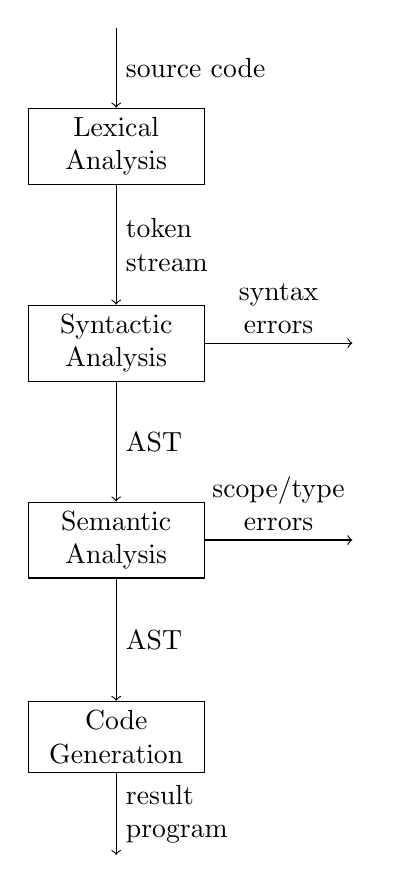
\begin{tikzpicture}
        \node[draw, text width=2cm, align=center] (LA) at (0, 0) {Lexical Analysis};
        \node[draw, text width=2cm, align=center] (SA) at (0, -2.5) {Syntactic Analysis};
        \node[draw, text width=2cm, align=center] (CA) at (0, -5) {Semantic Analysis};
        \node[draw, text width=2cm, align=center] (CG) at (0, -7.5) {Code \\ Generation};
        
        \draw[->] (0, 1.5) -- node[right] {source code} (LA);
        \draw[->] (LA) -- node[right, text width=2cm, align=left] {token \\ stream} (SA);
        
        \draw[->] (SA) -- node[above, text width=2cm, align=center] {syntax \\ errors} (3, -2.5);
        \draw[->] (SA) -- node[right] {AST} (CA);
        \draw[->] (CA) -- node[above, text width=2cm, align=center] {scope/type \\ errors} (3, -5);
        
        \draw[->] (CA) -- node[right] {AST} (CG);
        \draw[->] (CG) -- node[text width=2cm, align=left, right] {result \\ program} (0, -9);
    \end{tikzpicture}
    \caption{The data flow between the compilation phases.}
    \label{fig:compilation_process}
\end{figure}

We will now consider the different phases of the compilation process. This is summarised in Figure \ref{fig:compilation_process}. This figure, along with most of the content in this section, has been adapted from \cite{aho2007compilers}.

\subsection{Lexical Analysis}    
First, we perform \emph{lexical analysis}. In this stage, the source code is enriched to make it ready for parsing. In particular, we generate a stream of source code, which reads the program word by word. Then, it produces a stream of \emph{tokens}. A token is a word in source code along with a label. For instance, consider the mathematical expression \texttt{1 + 2}. We can convert this expression into 3 tokens: \texttt{(1, NUM)}, \texttt{(+, PLUS)} and \texttt{(2, NUM)}. 

\subsection{Syntactic Analysis}
Next, we try to parse the token stream into an (abstract) syntax tree (AST). If there are syntax errors present in the program, then it is not possible to construct a syntax tree. This will be detected during this phase, at which point we can throw a syntax error.

A syntax tree represents the program as a tree of nodes. Typically, the internal nodes represent operations and the leaves represent their arguments. An AST is a compact representation of a syntax tree that does not feature all the nodes. The abstract syntax tree for the expression \texttt{(1 + 2) * (3 + 4)} is given in Figure \ref{fig:AST_example}.

\begin{figure}[htb]
    \centering
    \begin{tikzpicture}[
        level 1/.style={sibling distance=4cm},
        level 2/.style={sibling distance=2cm},
    ]
        \node[ellipse, draw] {TIMES}
        child {
            node[ellipse, draw] {PLUS}
            child {
                node[draw] {\texttt{1}}
            }
            child {
                node[draw] {\texttt{2}}
            }
        }
        child {
            node[ellipse, draw] {PLUS}
            child {
                node[draw] {\texttt{3}}
            }
            child {
                node[draw] {\texttt{4}}
            }
        };
    \end{tikzpicture}
    \caption{The AST for the expression \texttt{(1 + 2) * (3 + 4)}}
    \label{fig:AST_example}
\end{figure}

There are many ways to parse the stream of tokens. A common method is \emph{recursive-descent} parsing. Here, we recursively parse the source code and generate nodes within the AST. For instance, we initially start by parsing a program. If we then encounter an expression, and this is allowed in the grammar of the language, we parse an expression. 

One way of recursive-descent parsing is by \emph{top-down} parsing. In this case, we produce the parent node of the AST and then generate its children. 

The simplest form of recursive-descent parsing is called \emph{predictive parsing}. This applies when the next token determines what structure it is to be parsed. For instance, if we see the token \texttt{if}, then we know we are parsing an \textit{if} command. Such a parser makes use of the \texttt{match} method- this is used to match the next token value.

% A snippet of a recursive-descent class \texttt{CodeParser} is given below, which illustrates how an if statement might be parsed.
% \begin{lstlisting}[language=TypeScript]
% class CodeParser {
%     parseIf():IfContext {
%         match("if");
%         var condition = parseExpr();
        
%         match("then");
%         var expr1 = parseExpr();
        
%         match("else");
%         var expr2 = parseExpr();

%         return new IfContext(condition, expr1, expr2);
%     }

%     // ... other parsing methods
% }
% \end{lstlisting}

\subsection{Semantic Analysis}
Now, we traverse the AST and check that there were no errors in the source code. Typically, there are 2 types of things to check in this stage- type and scope errors. 

In type errors, we check whether the AST has some type mismatch, e.g. \texttt{1 + true}. If there are no errors, then we will have assigned types to each variable. This information will likely be used during code generation.

In scope errors, we check whether some identifier present in code is undefined. To do so, we need to keep track of all the variables that are in scope at this point. In terms of functions, there is a design choice here- we can have all functions in scope from the start, or add them to scope as they are encountered. 

\subsection{Code Generation}
Finally, we convert the AST into code in the target language. In particular, we traverse the tree left-to-right and convert each phrase from the source language to the target. This can also be done using the visitor design pattern. Here, the return type is expected to be a representation of the target language.


%==================================================================================================================================
\chapter{Requirements}
% What is the problem that you want to solve, and how did you arrive at it?
% \section{Guidance}
% Make it clear how you derived the constrained form of your problem via a clear and logical process. 

% The analysis chapter explains the process by which you arrive at a concrete design. In software 
% engineering projects, this will include a statement of the requirement capture process and the
% derived requirements.

% In research projects, it will involve developing a design drawing on
% the work established in the background, and stating how the space of possible projects was
% sensibly narrowed down to what you have done.

%==================================================================================================================================
\chapter{Design}
\section{Language}

The TML provides commands to specify tape operations. In particular, 
\begin{itemize}
    \item we make use of \texttt{move} commands to move the tapehead pointer in some direction; and
    \item we make use of \texttt{changeto} commands to change the tapehead value to some letter in the alphabet.
\end{itemize}
To abstract states in a TM, the TML provides a PL-like alternative, called \emph{modules}. A module simulates a state in TMs. To allow for flow of code to go from one module to another, we make use of \texttt{goto} commands. We can go to the \textit{accept} and \textit{reject} states using the keywords \texttt{accept} and \texttt{reject} respectively.

The following illustrates a simple program in TML with all the basic operations.
\lstinputlisting[language=TML]{code/simple_program.txt}
The execution of a program starts at the first module, i.e. the module \texttt{first}. We remove the first tape value and move the tape pointer to the right. We then go to module \texttt{second} and continue execution. Note that we allow recursion- line 5 can be replaced with \texttt{goto first}.

To abstract the transition function, the language makes use of \emph{pattern-matching}. To resemble a traditional PL, we make use of \texttt{if} commands. This is shown in the example below.
\lstinputlisting[language=TML]{code/pattern_matching.txt}

Although the language is already equivalent to TMs, TML programs do not abstract TMs enough. In particular, modules are equivalent to TM states at this point. To mitigate this, we add nesting within \texttt{if} statements. That way, modules are more expressible than states. It also allows us to write programs that are more comparable to programs written in other languages. An example of a nested TML program is given below.
\lstinputlisting[language=TML]{code/isDiv2Rec.txt}
In this program, we have nested an \texttt{if} block within an \texttt{if} block in lines 12-16.

\begin{figure}[htb]
    \centering
    \begin{tikzpicture}
        \node[state, accepting] (q0) at (0, 0) {$q_0$};
        \node[state] (q1) at (2.5, -1.3) {$q_1$};
        \node[state, fill=green, opacity=0.6] (A) at (2.5, 1.3) {$A$};
        \node[state, fill=red, opacity=0.6] (R) at (5, -1.3) {$R$};

        \draw[->] (q0) -- node[above, rotate=20] {$0|\#, R$} (A);
        \draw[->] (q0) -- node[below, rotate=-20] {$1, R$} (q1);
        \draw[->] (q1) edge[loop below] node {$0|1, R$} (q1);
        \draw[->] (q1) -- node[below] {$\#, L$} (R);
    \end{tikzpicture}
    \caption{A TM with a self-loop at the state $q_1$.}
    \label{fig:self-loop-TM}
\end{figure}
Although nesting has made the language more like a typical PL, this is not enough. In particular, if we have a self-loop at a non-starting state, then the program cannot be written compactly. To see this, consider the TM at Figure \ref{fig:self-loop-TM}. Currently, the following is the only way to convert this TM into a TML program.
\lstinputlisting[language=TML]{code/forced_complete_program.txt}
What we have is a \emph{complete program}- this is a class of TML programs that are used to \textit{represent} TMs. In particular, 
\begin{itemize}
    \item there is a bijection between TMs and complete TML programs, and
    \item we can easily convert a module to a state, and vice versa.
\end{itemize}
It is not possible to combine the 2 modules- because the block corresponding to $q_1$ would be nested within $q_0$, recursion would convert the self-loop at $q_1$ into a transition from $q_1$ to $q_0$. By only allowing the TM to be written this way, we would not have completely abstracted TM states. We \textit{must} support nested self-loops.

To allow for self-loops to be nested, we introduce a new construct- a \texttt{while} command. This is similar to an \texttt{if} command, but after the block is executed, we stay at the same block. Note that this does not necessarily mean that the same \textit{case} is run. This is precisely a self-loop. We can now convert the TM to a single module:
\lstinputlisting[language=TML]{code/while_program.txt}
We can also conclude that the TML is not a mere \textit{representation} for TMs- we have found 2 programs that convert to the TM at Figure \ref{fig:self-loop-TM}. So, there is no bijection between TML programs and TMs. We have successfully abstracted TM states and transitions from the language!

The formal syntax of the language is given in the appendix, along with a proof of equivalence between TMs and TML programs with respect to tape execution. The proof of equivalence is composed of several proofs, which involve:
\begin{itemize}
    \item converting a TM into a (complete) TML program;
    \item converting a valid TML program into a complete TML program; and
    \item converting a complete TML program into a TM program.
\end{itemize}

\section{Parser}
The parser takes a program in TML and produces a corresponding TM. It also allows for the execution of a TML program, and a TM, on a tape. It does so in many steps.

\subsection{Lexical Analysis}
The first stage of parsing is lexical analysis, where we produce a stream of tokens from the source code. Since the TML is quite simple, this was decided to be unnecessary- we make use of a stream of \emph{source code}.

\subsection{Syntactic Analysis}

\begin{figure}[htb]
    \centering
    \begin{tikzpicture}[
        level 1/.style={sibling distance=4.5cm}
    ]
        \node[draw, ellipse] {PROGRAM}
        child[
            level 2/.style={sibling distance=1cm}
        ] {
            node[draw, ellipse] {ALPHABET}
            child {
                node[draw] {\texttt{a}}
            }
            child {
                node[draw] {\texttt{b}}
            }
        }
        child[
            level 2/.style={sibling distance=3cm}
        ] {
            node[draw, ellipse] {MODULE}
            child {
                node[draw] {\texttt{first}}
            }
            child {
                node[draw, ellipse] {BASIC-BLOCK}
                child {
                    node[draw, ellipse] {CHANGETO}
                    child {
                        node[draw] {\texttt{blank}}
                    }
                }
                child {
                    node[draw, ellipse] {MOVE}
                    child {
                        node[draw] {\texttt{left}}
                    }
                }
            }
        };
    \end{tikzpicture}
    \caption{An AST for the TML program with a module called \texttt{first}.}
    \label{fig:TML_AST}
\end{figure}

Next, the stream of source code is parsed into an AST. The AST has a node for each command. We illustrate this process with an example. So, assume we have the following source code.
\begin{lstlisting}[language=TML]
alphabet={a, b}
module first {
    changeto blank
    move left
}
\end{lstlisting}
Then, the parsing process results in the construction of the AST given in Figure \ref{fig:TML_AST}. 

The parser is top-down in nature. In particular, when parsing the program above, we try to construct the AST from the root and then fill out the branches and the leaves. Because the language does not have complex parsing rules, we also make use of predictive parsing. In particular, we construct the AST given above as follows:
\begin{enumerate}
    \item We first parse it as a program and construct the root node of the AST;
    \item We detect the alphabet at line 1, so we construct the alphabet branch in the AST; and 
    \item We parse the module \texttt{first} from line 2- we construct the module branch and parse its body.
\end{enumerate}
If successful, this process will result in an AST.

If the parser cannot construct an AST, then the program has some syntax error. In that case, the parser throws an error with a clear and a succinct message.

\subsection{Semantic Analysis}
After the AST has been constructed, we perform semantic analysis. The TML does not have a type system, meaning that we do not need to do type checking. On the other hand, the language makes use of identifiers, e.g. module names. So, we perform scope checking in this stage. This is done by traversing the AST once.

During this phase, we ensure that a \texttt{goto} command refers to a module that is already present in code. By design, we allow the module to be defined anywhere within the document. Moreover, we check that a module is not defined twice, and is not called \texttt{accept} or \texttt{reject}. We also validate that the letter of a \texttt{changeto} command is one of the letters in the \texttt{alphabet} or \texttt{blank}. 

Moreover, there is also a check to ensure that a switch block contains precisely one case for each letter in the alphabet. That is,
\begin{itemize}
    \item there are no duplicate cases present, and 
    \item the cases check all the letters, including \texttt{blank}.
\end{itemize}

\subsection{TM Generation}
Next, the AST is used to generate a TM. This is the final stage of the compilation process. There are many choices to represent a TM, including the formal definition of TMs and the FSM representation. To allow for more flexibility during code execution, the formal definition of TMs was chosen. 

This process is different to the one described in the proof of equivalence- here, we are directly converting a valid TML program into a TM. In essence, we have combined the two steps given in the proof to achieve this.

Initially, we define a TM. During the traversal of the AST, we add relevant states and transitions. This mostly takes place when we are at a block, either inside a \textit{module} or an \textit{if} command. The process depends on the type of block we have:
\begin{itemize}
    \item if we have a \textit{switch} block, then we define the transition function for each letter by visiting all the cases within the block;
    \item if we have a \textit{basic} block, then we define the transition function for all the letters in one go.
\end{itemize}
We have commands within the block/case that we can use to define the transition. For instance, if we have the command \texttt{move left}, then the transition direction will be left. If the command is not present, then we add the default transition, as specified in the language specification.

\subsection{TML Execution}

The AST is also used for executing a TML program on a tape. This is the final stage of the interpretation process. Since a TML program is compiled to a TM, this stage could have been avoided- we could make use of executing TM on a tape. However, this was also included since the execution of a TML program was thought to be more efficient. This is because TML program abstracts TM operations. For example, in TMs, each letter in a state should have a different transition, whereas TML supports the same transition for every letter.

The execution of a TML program follows the rules given in the specification. This is included in the appendix. Similarly, the execution of a TM follows the rules given in the background section.

\section{Product}
\subsection{Structure}
The website was planned to have multiple pages, which included:
\begin{itemize}
    \item the \emph{homepage} that allows the user to make use of the parser;
    \item the \emph{documentation pages} that explains TMs and TML programs; along with
    \item the \emph{error pages} to illustrate syntax and validation (non-syntax) errors.
\end{itemize}

A screenshot of the homepage is given in Figure \ref{fig:homepage_design}. More screenshots are given in the appendix.

\subsubsection{Homepage}
\begin{figure}[htb]
    \centering
    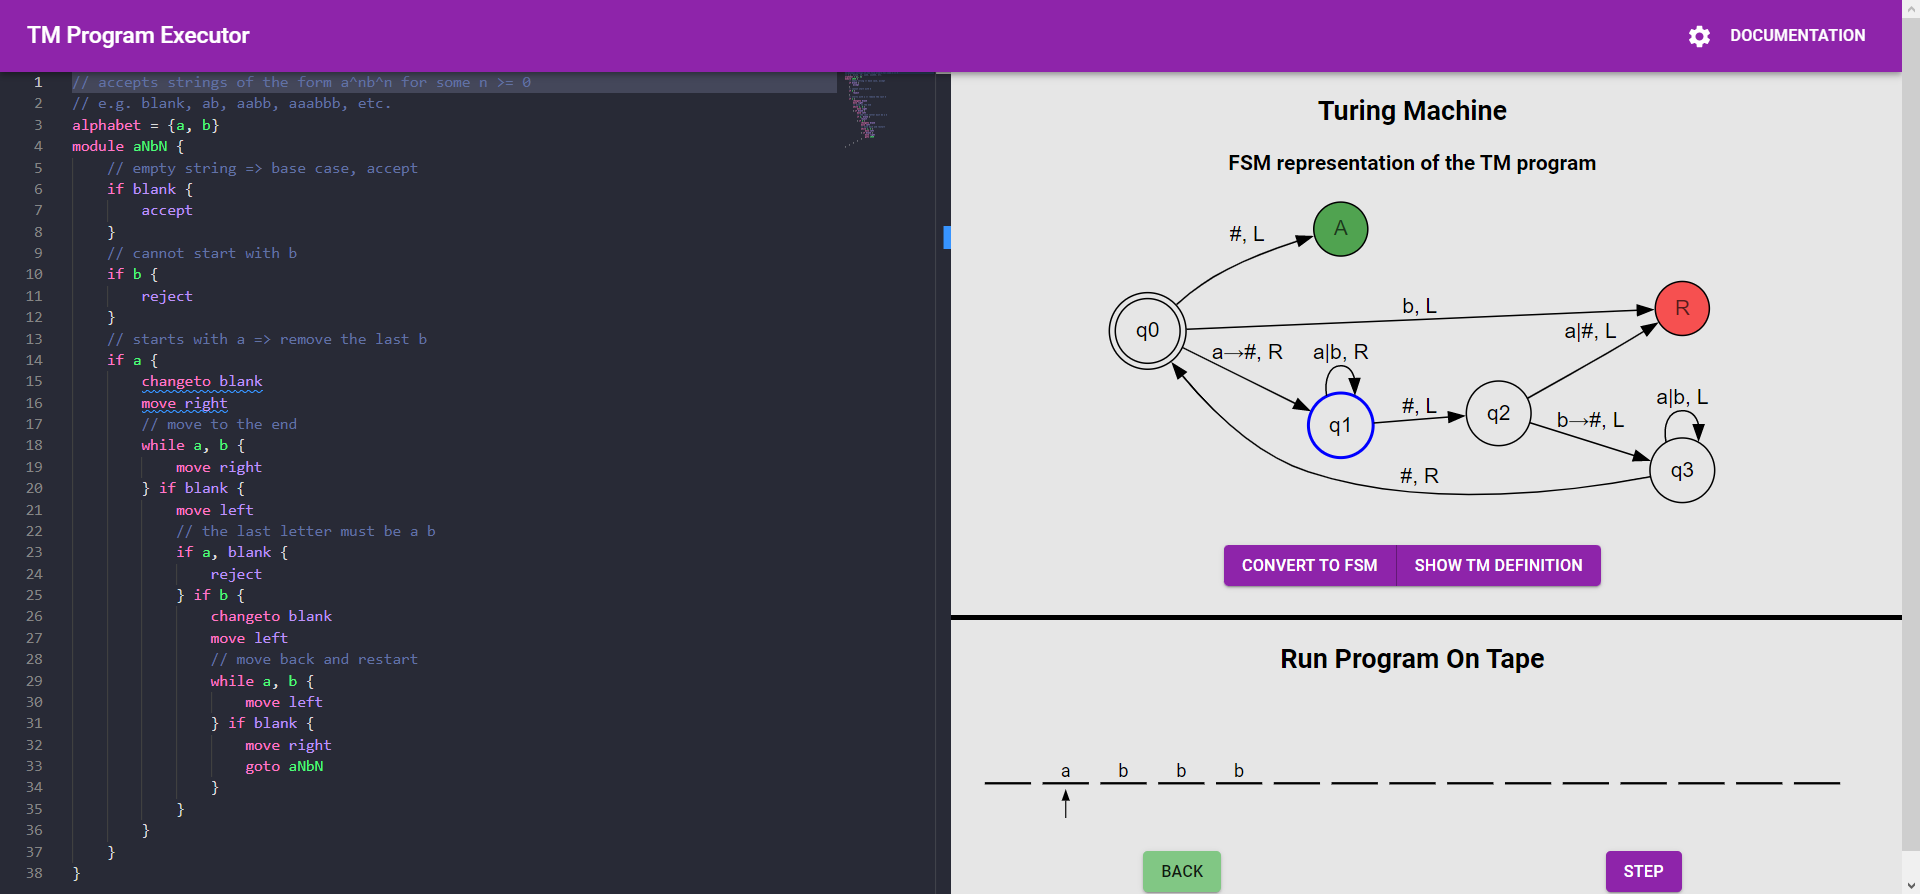
\includegraphics[scale=0.18]{images/Homepage execution start.png}
    \caption{The website homepage.}
    \label{fig:homepage_design}
\end{figure}

The user can input a program to the editor. If the program is valid, it can be compiled to a TM in two ways- it can either be converted to a FSM or to the definition version. The user can also execute the program on a tape after inputting a value. The step button performs one step in execution. 

The toolbar features a button to go to the documentation pages. There is also a button that allows the user to configure the page, e.g. fill the editor with some example code, change the editor theme, change font size, etc. 

\subsubsection{Documentation Pages}
The website has documentation pages that define both TMs and TML programs. In particular, the page:
\begin{itemize}
    \item gives the formal definition, 
    \item shows an example and 
    \item allows the user to execute the example on a tape.
\end{itemize}

\subsubsection{Error Pages}
For every language error, there is a dedicated page that:
\begin{itemize}
    \item describes the error informally;
    \item illustrates the error with an example program; and 
    \item presents a way to resolve the error.
\end{itemize}
There is also a general error page that lists all these errors.

The website makes use of \emph{Material Design}\footnote{\url{https://m3.material.io}}. The Material design provides common-purpose components, such as toolbars and icons. Moreover, Material design is quite widespread since all Google products make use of it. Hence, the user is expected to recognise these common constructs and should be able to easily interact with them. For instance, the user can recognise that a settings icon allows them to customise the website in some way. Furthermore, Material Design helps keep the website design responsive and consistent.

\subsection{TM Conversion}
The website supports live conversion of a TML program into a TM. The user can convert the TML program into both the FSM representation of a TM and its definition.

\begin{table}[htb]
    \centering
    \begin{tabular}{c|ccc}
        & $0$ & $1$ & $\#$ \\
        \hline
        $q_0$ & $(R, 0, q_0)$ & $(R, 1, q_0)$ & $(L, \#, q_1)$ \\
        $q_1$ & $(L, 0, q_A)$ & $(L, 1, q_R)$ & $(L, 1, q_R)$ 
    \end{tabular}
    \caption{A transition table.}
    \label{tbl:table_isDiv2}
\end{table}

The formal definition of the TM defines all the states and then presents the transitions in a table, such as the one in Table \ref{tbl:table_isDiv2}. In this example, the non-terminating states are $q_0$ and $q_1$, and the alphabet $\Sigma = \{0, 1\}$. Moreover, the transition table says that $\delta(q_0, 0) = (R, 0, q_0)$, meaning that, during execution:
\begin{itemize}
    \item the tapehead pointer moves to the \emph{right};
    \item the tapehead value stays $\emph{0}$; and 
    \item the current state remains $\emph{q}_\emph{0}$
\end{itemize}

\subsection{Tape Execution}
The user can input a valid string in the alphabet and execute the TML program on a tape. A valid string consists of letters in the alphabet and the blank symbol. The tape panel features 15 visible tape entries (positions for an input value). The tape panel animates the execution process in the tape entries, which involves:
\begin{itemize}
    \item changing the tapehead value; and
    \item moving the tape to the left or the right.
\end{itemize}
Note that a \textit{move} command moves the \textit{pointer}, not the tape. Hence, the command \texttt{move left} moves the tape to the \textit{right}; the tapehead position remains constant.

\begin{figure}[htb]
    \centering
    \begin{subfigure}{0.3\textwidth}
        \centering
        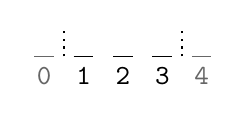
\begin{tikzpicture}
            \foreach \x in {0, 4} {
                \draw[opacity=0.6] (\x*0.5, 0) -- (\x*0.5+0.25, 0);
                \node[opacity=0.6] at (\x*0.5+0.125, -0.25) {\texttt{\x}};
            }
            \foreach \x in {1, 2, 3} {
                \draw (\x*0.5, 0) -- (\x*0.5+0.25, 0);
                \node at (\x*0.5+0.125, -0.25) {\texttt{\x}};
            }

            \draw[thick, dotted] (0.375, 0) -- (0.375, 0.35);
            \draw[thick, dotted] (1.875, 0) -- (1.875, 0.35);
        \end{tikzpicture}
        \caption{}
    \end{subfigure}
    \hfill
    \begin{subfigure}{0.3\textwidth}
        \centering
        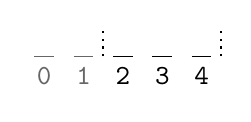
\begin{tikzpicture}
            \foreach \x in {0, 1} {
                \draw[opacity=0.6] (\x*0.5, 0) -- (\x*0.5+0.25, 0);
                \node[opacity=0.6] at (\x*0.5+0.125, -0.25) {\texttt{\x}};
            }
            \foreach \x in {2, 3, 4} {
                \draw (\x*0.5, 0) -- (\x*0.5+0.25, 0);
                \node at (\x*0.5+0.125, -0.25) {\texttt{\x}};
            }

            \draw[thick, dotted] (0.875, 0) -- (0.875, 0.35);
            \draw[thick, dotted] (2.375, 0) -- (2.375, 0.35);
        \end{tikzpicture}
        \caption{}
    \end{subfigure}
    \hfill
    \begin{subfigure}{0.3\textwidth}
        \centering
        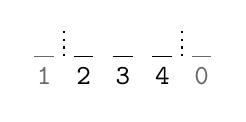
\begin{tikzpicture}
            \foreach \x[evaluate={int(mod(\x, 5))} as \y] in {5, 1} {
                \draw[opacity=0.6] (\x*0.5, 0) -- (\x*0.5+0.25, 0);
                \node[opacity=0.6] at (\x*0.5+0.125, -0.25) {\texttt{\y}};
            }

            \foreach \x in {2, 3, 4} {
                \draw (\x*0.5, 0) -- (\x*0.5+0.25, 0);
                \node at (\x*0.5+0.125, -0.25) {\texttt{\x}};
            }

            \draw[thick, dotted] (0.875, 0) -- (0.875, 0.35);
            \draw[thick, dotted] (2.375, 0) -- (2.375, 0.35);
        \end{tikzpicture}
        \caption{}
    \end{subfigure}
    \caption{The transition process for tape entries.}
    \label{fig:tape_movement}
\end{figure}

For the tape movement animation to look smooth, there are always 2 tape entries to either side of the tape. That way, if the tape gets moved left or right, there will be a tape entry to show. This is illustrated in Figure \ref{fig:tape_movement} (a)- the tape entries 0 and 4 are out of frame and therefore invisible. 

When the tape moves, there will be 2 tape entries on one side. For instance, if the tape moves to the left in Figure \ref{fig:tape_movement} (a), we get Figure \ref{fig:tape_movement} (b)- there are 2 invisible entries to the left. After the transition has completed, we move the most extreme tape entry to the other side. In the example, we move tape entry 0 to the right, leading to the tape state given in Figure \ref{fig:tape_movement} (c). At this point, we also change the tape value of entry 0 so that it matches the value at index 5. Since these changes are invisible, they take place instantly after the animation is complete.


%==================================================================================================================================
\chapter{Implementation}
% What did you do to implement this idea, and what technical achievements did you make?
% \section{Guidance}
% You can't talk about everything. Cover the high level first, then cover important, relevant or impressive details.

% \section{General guidance for technical writing}

% These points apply to the whole dissertation, not just this chapter.

% \subsection{Figures}
% \emph{Always} refer to figures included, like Figure \ref{fig:relu}, in the body of the text. Include full, explanatory captions and make sure the figures look good on the page.
% You may include multiple figures in one float, as in Figure \ref{fig:synthetic}, using \texttt{subcaption}, which is enabled in the template.


% Figures are important. Use them well.
% \begin{figure}[htb]
%     \centering
%     \includegraphics[width=0.5\linewidth]{images/relu.pdf}    

%     \caption{In figure captions, explain what the reader is looking at: ``A schematic of the rectifying linear unit, where $a$ is the output amplitude,
%     $d$ is a configurable dead-zone, and $Z_j$ is the input signal'', as well as why the reader is looking at this: 
%     ``It is notable that there is no activation \emph{at all} below 0, which explains our initial results.'' 
%     \textbf{Use vector image formats (.pdf) where possible}. Size figures appropriately, and do not make them over-large or too small to read.
%     }

%     % use the notation fig:name to cross reference a figure
%     \label{fig:relu} 
% \end{figure}


% \begin{figure}[htb] 
%     \centering
%     \begin{subfigure}[b]{0.45\textwidth}
%         \includegraphics[width=\textwidth]{images/synthetic.png}
%         \caption{Synthetic image, black on white.}
%         \label{fig:syn1}
%     \end{subfigure}
%     ~ %add desired spacing between images, e. g. ~, \quad, \qquad, \hfill etc. 
%       %(or a blank line to force the subfigure onto a new line)
%     \begin{subfigure}[b]{0.45\textwidth}
%         \includegraphics[width=\textwidth]{images/synthetic_2.png}
%         \caption{Synthetic image, white on black.}
%         \label{fig:syn2}
%     \end{subfigure}
%     ~ %add desired spacing between images, e. g. ~, \quad, \qquad, \hfill etc. 
%     %(or a blank line to force the subfigure onto a new line)    
%     \caption{Synthetic test images for edge detection algorithms. \subref{fig:syn1} shows various gray levels that require an adaptive algorithm. \subref{fig:syn2}
%     shows more challenging edge detection tests that have crossing lines. Fusing these into full segments typically requires algorithms like the Hough transform.
%     This is an example of using subfigures, with \texttt{subref}s in the caption.
%     }\label{fig:synthetic}
% \end{figure}

% \clearpage

% \subsection{Equations}

% Equations should be typeset correctly and precisely. Make sure you get parenthesis sizing correct, and punctuate equations correctly 
% (the comma is important and goes \textit{inside} the equation block). Explain any symbols used clearly if not defined earlier. 

% For example, we might define:
% \begin{equation}
%     \hat{f}(\xi) = \frac{1}{2}\left[ \int_{-\infty}^{\infty} f(x) e^{2\pi i x \xi} \right],
% \end{equation}    
% where $\hat{f}(\xi)$ is the Fourier transform of the time domain signal $f(x)$.

% \subsection{Algorithms}
% Algorithms can be set using \texttt{algorithm2e}, as in Algorithm \ref{alg:metropolis}.

% % NOTE: line ends are denoted by \; in algorithm2e
% \begin{algorithm}
%     \DontPrintSemicolon
%     \KwData{$f_X(x)$, a probability density function returing the density at $x$.\; $\sigma$ a standard deviation specifying the spread of the proposal distribution.\;
%     $x_0$, an initial starting condition.}
%     \KwResult{$s=[x_1, x_2, \dots, x_n]$, $n$ samples approximately drawn from a distribution with PDF $f_X(x)$.}
%     \Begin{
%         $s \longleftarrow []$\;
%         $p \longleftarrow f_X(x)$\;
%         $i \longleftarrow 0$\;
%         \While{$i < n$}
%         {
%             $x^\prime \longleftarrow \mathcal{N}(x, \sigma^2)$\;
%             $p^\prime \longleftarrow f_X(x^\prime)$\;
%             $a \longleftarrow \frac{p^\prime}{p}$\;
%             $r \longleftarrow U(0,1)$\;
%             \If{$r<a$}
%             {
%                 $x \longleftarrow x^\prime$\;
%                 $p \longleftarrow f_X(x)$\;
%                 $i \longleftarrow i+1$\;
%                 append $x$ to $s$\;
%             }
%         }
%     }
    
% \caption{The Metropolis-Hastings MCMC algorithm for drawing samples from arbitrary probability distributions, 
% specialised for normal proposal distributions $q(x^\prime|x) = \mathcal{N}(x, \sigma^2)$. The symmetry of the normal distribution means the acceptance rule takes the simplified form.}\label{alg:metropolis}
% \end{algorithm}

% \subsection{Tables}

% If you need to include tables, like Table \ref{tab:operators}, use a tool like https://www.tablesgenerator.com/ to generate the table as it is
% extremely tedious otherwise. 

% \begin{table}[]
%     \caption{The standard table of operators in Python, along with their functional equivalents from the \texttt{operator} package. Note that table
%     captions go above the table, not below. Do not add additional rules/lines to tables. }\label{tab:operators}
%     %\tt 
%     \rowcolors{2}{}{gray!3}
%     \begin{tabular}{@{}lll@{}}
%     %\toprule
%     \textbf{Operation}    & \textbf{Syntax}                & \textbf{Function}                            \\ %\midrule % optional rule for header
%     Addition              & \texttt{a + b}                          & \texttt{add(a, b)}                                    \\
%     Concatenation         & \texttt{seq1 + seq2}                    & \texttt{concat(seq1, seq2)}                           \\
%     Containment Test      & \texttt{obj in seq}                     & \texttt{contains(seq, obj)}                           \\
%     Division              & \texttt{a / b}                          & \texttt{div(a, b) }  \\
%     Division              & \texttt{a / b}                          & \texttt{truediv(a, b) } \\
%     Division              & \texttt{a // b}                         & \texttt{floordiv(a, b)}                               \\
%     Bitwise And           & \texttt{a \& b}                         & \texttt{and\_(a, b)}                                  \\
%     Bitwise Exclusive Or  & \texttt{a \textasciicircum b}           & \texttt{xor(a, b)}                                    \\
%     Bitwise Inversion     & \texttt{$\sim$a}                        & \texttt{invert(a)}                                    \\
%     Bitwise Or            & \texttt{a | b}                          & \texttt{or\_(a, b)}                                   \\
%     Exponentiation        & \texttt{a ** b}                         & \texttt{pow(a, b)}                                    \\
%     Identity              & \texttt{a is b}                         & \texttt{is\_(a, b)}                                   \\
%     Identity              & \texttt{a is not b}                     & \texttt{is\_not(a, b)}                                \\
%     Indexed Assignment    & \texttt{obj{[}k{]} = v}                 & \texttt{setitem(obj, k, v)}                           \\
%     Indexed Deletion      & \texttt{del obj{[}k{]}}                 & \texttt{delitem(obj, k)}                              \\
%     Indexing              & \texttt{obj{[}k{]}}                     & \texttt{getitem(obj, k)}                              \\
%     Left Shift            & \texttt{a \textless{}\textless b}       & \texttt{lshift(a, b)}                                 \\
%     Modulo                & \texttt{a \% b}                         & \texttt{mod(a, b)}                                    \\
%     Multiplication        & \texttt{a * b}                          & \texttt{mul(a, b)}                                    \\
%     Negation (Arithmetic) & \texttt{- a}                            & \texttt{neg(a)}                                       \\
%     Negation (Logical)    & \texttt{not a}                          & \texttt{not\_(a)}                                     \\
%     Positive              & \texttt{+ a}                            & \texttt{pos(a)}                                       \\
%     Right Shift           & \texttt{a \textgreater{}\textgreater b} & \texttt{rshift(a, b)}                                 \\
%     Sequence Repetition   & \texttt{seq * i}                        & \texttt{repeat(seq, i)}                               \\
%     Slice Assignment      & \texttt{seq{[}i:j{]} = values}          & \texttt{setitem(seq, slice(i, j), values)}            \\
%     Slice Deletion        & \texttt{del seq{[}i:j{]}}               & \texttt{delitem(seq, slice(i, j))}                    \\
%     Slicing               & \texttt{seq{[}i:j{]}}                   & \texttt{getitem(seq, slice(i, j))}                    \\
%     String Formatting     & \texttt{s \% obj}                       & \texttt{mod(s, obj)}                                  \\
%     Subtraction           & \texttt{a - b}                          & \texttt{sub(a, b)}                                    \\
%     Truth Test            & \texttt{obj}                            & \texttt{truth(obj)}                                   \\
%     Ordering              & \texttt{a \textless b}                  & \texttt{lt(a, b)}                                     \\
%     Ordering              & \texttt{a \textless{}= b}               & \texttt{le(a, b)}                                     \\
%     % \bottomrule
%     \end{tabular}
%     \end{table}
% \subsection{Code}

% Avoid putting large blocks of code in the report (more than a page in one block, for example). Use syntax highlighting if possible, as in Listing \ref{lst:callahan}.

% \begin{lstlisting}[language=python, float, caption={The algorithm for packing the $3\times 3$ outer-totalistic binary CA successor rule into a 
%     $16\times 16\times 16\times 16$ 4 bit lookup table, running an equivalent, notionally 16-state $2\times 2$ CA.}, label=lst:callahan]
%     def create_callahan_table(rule="b3s23"):
%         """Generate the lookup table for the cells."""        
%         s_table = np.zeros((16, 16, 16, 16), dtype=np.uint8)
%         birth, survive = parse_rule(rule)

%         # generate all 16 bit strings
%         for iv in range(65536):
%             bv = [(iv >> z) & 1 for z in range(16)]
%             a, b, c, d, e, f, g, h, i, j, k, l, m, n, o, p = bv

%             # compute next state of the inner 2x2
%             nw = apply_rule(f, a, b, c, e, g, i, j, k)
%             ne = apply_rule(g, b, c, d, f, h, j, k, l)
%             sw = apply_rule(j, e, f, g, i, k, m, n, o)
%             se = apply_rule(k, f, g, h, j, l, n, o, p)

%             # compute the index of this 4x4
%             nw_code = a | (b << 1) | (e << 2) | (f << 3)
%             ne_code = c | (d << 1) | (g << 2) | (h << 3)
%             sw_code = i | (j << 1) | (m << 2) | (n << 3)
%             se_code = k | (l << 1) | (o << 2) | (p << 3)

%             # compute the state for the 2x2
%             next_code = nw | (ne << 1) | (sw << 2) | (se << 3)

%             # get the 4x4 index, and write into the table
%             s_table[nw_code, ne_code, sw_code, se_code] = next_code

%         return s_table

% \end{lstlisting}

%==================================================================================================================================
\chapter{Evaluation} 
% How good is your solution? How well did you solve the general problem, and what evidence do you have to support that?

% \section{Guidance}
% \begin{itemize}
%     \item
%         Ask specific questions that address the general problem.
%     \item
%         Answer them with precise evidence (graphs, numbers, statistical
%         analysis, qualitative analysis).
%     \item
%         Be fair and be scientific.
%     \item
%         The key thing is to show that you know how to evaluate your work, not
%         that your work is the most amazing product ever.
% \end{itemize}

% \section{Evidence}
% Make sure you present your evidence well. Use appropriate visualisations, 
% reporting techniques and statistical analysis, as appropriate. The point is not
% to dump all the data you have but to present an argument well supported by evidence gathered.

% If you use numerical evidence, specify reasonable numbers of significant digits; don't state ``18.41141\% of users were successful'' if you only had 20 users. If you average \textit{anything}, present both a measure of central tendency (e.g. mean, median) \textit{and} a measure of spread (e.g. standard deviation, min/max, interquartile range).

% You can use \texttt{siunitx} to define units, space numbers neatly, and set the precision for the whole LaTeX document. 

% % setup siunitx to have two decimal places
% \sisetup{
% 	round-mode = places,
% 	round-precision = 2
% }

% For example, these numbers will appear with two decimal places: \num{3.141592}, \num{2.71828}, and this one will appear with reasonable spacing \num{1000000}.



% If you use statistical procedures, make sure you understand the process you are using,
% and that you check the required assumptions hold in your case. 

% If you visualise, follow the basic rules, as illustrated in Figure \ref{fig:boxplot}:
% \begin{itemize}
% \item Label everything correctly (axis, title, units).
% \item Caption thoroughly.
% \item Reference in text.
% \item \textbf{Include appropriate display of uncertainty (e.g. error bars, Box plot)}
% \item Minimize clutter.
% \end{itemize}

% See the file \texttt{guide\_to\_visualising.pdf} for further information and guidance.

% \begin{figure}[htb]
%     \centering
%     \includegraphics[width=1.0\linewidth]{images/boxplot_finger_distance.pdf}    

%     \caption{Average number of fingers detected by the touch sensor at different heights above the surface, averaged over all gestures. Dashed lines indicate
%     the true number of fingers present. The Box plots include bootstrapped uncertainty notches for the median. It is clear that the device is biased toward 
%     undercounting fingers, particularly at higher $z$ distances.
%     }

%     % use the notation fig:name to cross reference a figure
%     \label{fig:boxplot} 
% \end{figure}


%==================================================================================================================================
\chapter{Conclusion}    
% Summarise the whole project for a lazy reader who didn't read the rest (e.g. a prize-awarding committee). This chapter should be short in most dissertations; maybe one to three pages.
% \section{Guidance}
% \begin{itemize}
%     \item
%         Summarise briefly and fairly.
%     \item
%         You should be addressing the general problem you introduced in the
%         Introduction.        
%     \item
%         Include summary of concrete results (``the new compiler ran 2x
%         faster'')
%     \item
%         Indicate what future work could be done, but remember: \textbf{you
%         won't get credit for things you haven't done}.
% \end{itemize}

% \section{Summary}
% Summarise what you did; answer the general questions you asked in the introduction. What did you achieve? Briefly describe what was built and summarise the evaluation results.

% \section{Reflection}
% Discuss what went well and what didn't and how you would do things differently if you did this project again.

% \section{Future work}
% Discuss what you would do if you could take this further -- where would the interesting directions to go next be? (e.g. you got another year to work on it, or you started a company to work on this, or you pursued a PhD on this topic)

%==================================================================================================================================
%
% 
%==================================================================================================================================
%  APPENDICES  

\begin{appendices}
    \chapter{TML EBNF}
The following is the EBNF for the Turing Machine Language.
\begin{align*}
    \textit{program} &= \textit{alphabet} \ \textit{module}^+ \\
    \textit{alphabet} &= \texttt{alphabet} \ \texttt{=} \ \texttt{\{} \ \textit{seq-val} \ \texttt{\}} \\
    \textit{module} &= \texttt{module} \ \textit{id} \ \texttt{\{} \ \textit{block}^+ \ \texttt{\}} \\
    \textit{block} &= \textit{basic-block} \ | \ \textit{switch-block} \\
    \textit{switch-block} &= \texttt{switch tapehead \{} \ \textit{case-block}^+ \ \texttt{\}} \\
    \textit{case-block} &= \textit{if-block} \ | \ \textit{while-block} \\
    \textit{if-block} &= \texttt{if} \ \textit{seq-val} \ \texttt{\{} \textit{block}^+ \texttt{\}} \\
    \textit{while-block} &= \texttt{while} \ \textit{seq-val} \ \texttt{\{} \ \textit{core-com}^+ \ \texttt{\}} \\
    \textit{basic-block} &= (\textit{core-com} \ | \ \textit{flow-com})^+ \\
    \textit{core-com} &= \texttt{move} \ \textit{direction} \ | \ \texttt{changeto} \ \textit{value} \\
    \textit{flow-com} &= \texttt{goto} \ \textit{id} \ | \ \textit{terminate} \\
    \textit{terminate} &= \texttt{reject} \ | \ \texttt{accept} \\
    \textit{direction} &= \texttt{left} \ | \ \texttt{right} \\
    \textit{seq-val} &= (\textit{value} \texttt{,})^* \ \textit{value} \\
    \textit{value} &= \texttt{blank} \ | \ \texttt{a} \ | \ \texttt{b} \ | \ \texttt{c} \ | \ \dots \ | \ \texttt{z} \ | \ \texttt{0} \ | \ \texttt{1} \ | \ \dots \ | \ \texttt{9} \\
    \textit{id} &= (\texttt{a} \ | \ \texttt{b} \ | \ \texttt{c} \ | \ \dots \ | \ \texttt{z} \ | \ \texttt{A} \ | \ \texttt{B} \ | \ \texttt{C} \ | \ \dots \ | \ \texttt{Z})^+
\end{align*}
    \chapter{Incorrect TML Programs}

Below is a selection of incorrect TML programs, along with an explanation as to why they are incorrect.
\begin{itemize}
    \item \textbf{Invalid while block (flow command)}
\begin{lstlisting}[language=TML]
alphabet = {a, b}
module main {
    while a, b {
        accept
    }
}
\end{lstlisting}
    A while block cannot have a flow command. We know that the next block to be executed is the same block, so this doesn't make sense- are we meant to terminate or re-run the current block?

    \item \textbf{Invalid while block (multiple blocks)}
\begin{lstlisting}[language=TML]
alphabet = {a, b}
module main {
    while blank {
        move left
        move right
    }
}
\end{lstlisting}
    A while block must be composed of a single basic block. We know that a while block corresponds to a self-loop, so if we have 2 blocks, we would need another state to link to the current state. This doesn't make sense, so we can only have one block. The block must also be a simple block since we have already fixed what character the while block applies to.

    \item \textbf{Invalid switch block (first block not basic)}
\begin{lstlisting}[language=TML]
alphabet = {a, b}
module main {
    if a, blank {
        if a {
            move right
        }
    }
}
\end{lstlisting}
    The first block in a switch block must be a basic block. That is, we cannot have nested if blocks without an intermediate command. This does not make sense semantically- in the case above, we should just have a single if block for \texttt{a}.

    \item \textbf{Invalid module (flow command not final)}
\begin{lstlisting}[language=TML]
alphabet = {a, b}
module main {
    goto simple
    move left
}
module simple {
    reject
}
\end{lstlisting}
    If we have a \emph{flow}-command in a block, then it must be the final command. A \emph{flow}-command moves to terminating execution or executing a module from the start, so any command below it cannot be executed. In this case, we are moving to a different block called \texttt{simple}, so we never move \texttt{left}.

    \item \textbf{Invalid module (switch block not final)}
\begin{lstlisting}[language=TML]
alphabet = {a, b}
module a {
    if a, b {
        changeto blank
        move right
        move right
        changeto b
    } if blank {
        move left
        changeto a
        reject
    }
    accept
}
\end{lstlisting}
    If a module has a \textit{switch} block, it must be the final block. In this case, that is not the case. It is possible that the program is meant to accept if we execute the \textit{if}-block at line 3, but it is not possible to continue the \textit{if}-block at line 8- this block already ends with a flow command. So, the execution would be unclear if this was allowed.

    \item \textbf{Invalid module (invalid name)}
\begin{lstlisting}[language=TML]
alphabet = {a, b}
module accept {
    move right
}
\end{lstlisting}
    A module cannot be named \texttt{accept} or \texttt{reject}. It can be named any of the other keywords, but not \texttt{accept} or \texttt{reject}.

\end{itemize}

    \chapter{TML Examples}
\section{Executing a TML program on a Tape}
Consider the following TML program:
\begin{lstlisting}[language=TML]
alphabet = {"a", "b"}
module palindrome {
    if blank {
        accept
    } if a {
        changeto blank
        move right
        while a, b {
            move right
        } if blank {
            move left
            if blank, a {
                changeto blank
                move left
                goto restart
            } if b {
                reject
            }
        }
    }  if b {
        changeto blank
        move right
        while a, b {
            move right
        } if blank {
            move left
            if blank, b {
                changeto blank
                move left
                goto restart
            } if a {
                reject
            }
        }
    }
}
module restart {
    while a, b {
        move left
    } if blank {
        move right
        goto palindrome
    }
}
\end{lstlisting}
We will execute the program on the following tape.
\begin{figure}[H]
    \centering
    \begin{tikzpicture}
        \draw[thick] (-0.25, 0) -- (0, 0);
        \foreach \x[count=\i] in {a, b, a} {
            \draw[thick] (\i*0.5-0.25, 0) -- (\i*0.5, 0);
            \node at (\i*0.5-0.125, 0.3) {\texttt{\x}};
        }
        \draw[thick] (1.75, 0) -- (2, 0);

        \draw[->, thick] (0.375, -0.5) -- (0.375, -0.1);
    \end{tikzpicture}
\end{figure}
\noindent The arrow points at the tapehead value. We first execute the first block in the module \texttt{palindrome}. Since the tapehead value is \texttt{a}, we execute the basic block at lines 5-20. So, we change the tapehead value to \texttt{blank}, and the tapehead moves to the right by one step. Since this is an \textit{if}-block, without a flow command, and there is a block following this one, the next block to be executed is the switch block at lines 8-19. Now, the current tape is the following.
\begin{figure}[H]
    \centering
    \begin{tikzpicture}
        \draw[thick] (-0.25, 0) -- (0, 0);
        \foreach \x[count=\i] in {b, a} {
            \draw[thick] (\i*0.5-0.25, 0) -- (\i*0.5, 0);
            \node at (\i*0.5-0.125, 0.3) {\texttt{\x}};
        }
        \draw[thick] (1.25, 0) -- (1.5, 0);

        \draw[->, thick] (0.375, -0.5) -- (0.375, -0.1);
    \end{tikzpicture}
\end{figure}
\noindent The current block is a switch block. The tapehead value is \texttt{b}, so we are at the \textit{while} command at line 9. The basic block here only contains a \textit{move} command. So, we leave the tape as is, and the tapehead moves to the right once. This is a \textit{while} command, so the next block to execute is still this switch block. The current tape state is the following.
\begin{figure}[H]
    \centering
    \begin{tikzpicture}
        \draw[thick] (-0.25, 0) -- (0, 0);
        \foreach \x[count=\i] in {b, a} {
            \draw[thick] (\i*0.5-0.25, 0) -- (\i*0.5, 0);
            \node at (\i*0.5-0.125, 0.3) {\texttt{\x}};
        }
        \draw[thick] (1.25, 0) -- (1.5, 0);

        \draw[->, thick] (0.875, -0.5) -- (0.875, -0.1);
    \end{tikzpicture}
\end{figure}
\noindent The current block is still a switch block. The tapehead value is \texttt{a}, so we execute the same \textit{while} command at line 9. Moreover, the next block to execute is still the switch block. Now, the current tape state is the following.
\begin{figure}[H]
    \centering
    \begin{tikzpicture}
        \draw[thick] (-0.25, 0) -- (0, 0);
        \foreach \x[count=\i] in {b, a} {
            \draw[thick] (\i*0.5-0.25, 0) -- (\i*0.5, 0);
            \node at (\i*0.5-0.125, 0.3) {\texttt{\x}};
        }
        \draw[thick] (1.25, 0) -- (1.5, 0);

        \draw[->, thick] (1.375, -0.5) -- (1.375, -0.1);
    \end{tikzpicture}
\end{figure}
\noindent For the third time, we are executing the same switch block. Now, however, the tapehead value is \texttt{blank}, so we execute the first block of the \textit{if} command at line 5, i.e. we move to the left. Since this is an \textit{if} command and this is not the last block in the if command, the next block to execute is the switch block at lines 12-18.
\begin{figure}[H]
    \centering
    \begin{tikzpicture}
        \draw[thick] (-0.25, 0) -- (0, 0);
        \foreach \x[count=\i] in {b, a} {
            \draw[thick] (\i*0.5-0.25, 0) -- (\i*0.5, 0);
            \node at (\i*0.5-0.125, 0.3) {\texttt{\x}};
        }
        \draw[thick] (1.25, 0) -- (1.5, 0);

        \draw[->, thick] (0.875, -0.5) -- (0.875, -0.1);
    \end{tikzpicture}
\end{figure}
\noindent Now, the current block is a switch block. The tapehead value is \texttt{a}, so we take the basic block at lines 12-16. The value of the tapehead becomes \texttt{blank}, and moves to the left. The next block to execute is the switch block in \texttt{restart}.
\begin{figure}[H]
    \centering
    \begin{tikzpicture}
        \draw[thick] (-0.25, 0) -- (0, 0);
        \foreach \x[count=\i] in {b} {
            \draw[thick] (\i*0.5-0.25, 0) -- (\i*0.5, 0);
            \node at (\i*0.5-0.125, 0.3) {\texttt{\x}};
        }
        \draw[thick] (0.75, 0) -- (1, 0);

        \draw[->, thick] (0.375, -0.5) -- (0.375, -0.1);
    \end{tikzpicture}
\end{figure}
\noindent Since the current tapehead value is \texttt{b}, we execute the basic block at line 39. So, we move to the left, and the tape is left as is. Moreover, since this is a while block, the next block to execute is still the switch block.
\begin{figure}[H]
    \centering
    \begin{tikzpicture}
        \draw[thick] (-0.25, 0) -- (0, 0);
        \foreach \x[count=\i] in {b} {
            \draw[thick] (\i*0.5-0.25, 0) -- (\i*0.5, 0);
            \node at (\i*0.5-0.125, 0.3) {\texttt{\x}};
        }
        \draw[thick] (0.75, 0) -- (1, 0);

        \draw[->, thick] (-0.125, -0.5) -- (-0.125, -0.1);
    \end{tikzpicture}
\end{figure}
\noindent Since the current tapehead state is \texttt{blank}, we execute the basic block at lines 40-43. So, we move to the left, and the tape is left as is. The next block to execute is the switch block at \texttt{palindrome}.
\begin{figure}[H]
    \centering
    \begin{tikzpicture}
        \draw[thick] (-0.25, 0) -- (0, 0);
        \foreach \x[count=\i] in {b} {
            \draw[thick] (\i*0.5-0.25, 0) -- (\i*0.5, 0);
            \node at (\i*0.5-0.125, 0.3) {\texttt{\x}};
        }
        \draw[thick] (0.75, 0) -- (1, 0);

        \draw[->, thick] (0.375, -0.5) -- (0.375, -0.1);
    \end{tikzpicture}
\end{figure}
\noindent Since the current tapehead state is \texttt{b}, we execute the basic block at lines 21-22. So, we change the tapehead value to \texttt{blank}, move to the right. This is a while block, so the next block to be executed is still the switch block.
\begin{figure}[H]
    \centering
    \begin{tikzpicture}
        \draw[thick] (-0.25, 0) -- (0, 0);
        \draw[thick] (0.25, 0) -- (0.5, 0);
        \draw[thick] (0.75, 0) -- (1, 0);

        \draw[->, thick] (0.875, -0.5) -- (0.875, -0.1);
    \end{tikzpicture}
\end{figure}
\noindent At this point, the tapehead index moves between the blank values as we move to the basic block at line 3. Then, the execution terminates and we accept the tape.

\section{Completing a TML program}
The steps to convert a TML program to complete it is the following:
\begin{enumerate}
    \item We first break each module into smaller modules so that every module has just one basic/switch block- we add a \textit{goto} command to the next module if it appeared just below this block.
    \item Then, we can convert each basic block to a switch block by just adding a single case that applies to each letter in the alphabet.
    \item Finally, we add the default values to each basic block to get a complete TML program.
\end{enumerate}

We illustrate this with an example. Assume we first have the following program.
\begin{lstlisting}[language=TML]
alphabet = {"a", "b"}
module simpleProgram {
    changeto b
    move left
    move right
    accept
}
\end{lstlisting}
After applying step 1 of completion, we get the following program.
\begin{lstlisting}[language=TML]
alphabet = {"a", "b"}
module simple1 {
    changeto b
    move left
    goto simple2
}
module simple2 {
    move right
    accept
}
\end{lstlisting}
After applying step 2, we have the following program.
\begin{lstlisting}[language=TML]
alphabet = {"a", "b"}
module simple1 {
    if a, b, blank {
        changeto b
        move left
        goto simple2
    }
}
module simple2 {
    if a, b, blank {
        move right
        accept
    }
}
\end{lstlisting}
Finally, after applying step 3, we get the following program:
\begin{lstlisting}[language=TML]
alphabet = {"a", "b"}
module simple1 {
    if a {
        changeto b
        move left
        goto simple2
    } if b {
        changeto b
        move left
        goto simple2
    } if blank {
        changeto b
        move left
        goto simple2
    }
}
module simple2 {
    if a {
        changeto a
        move right
        accept
    } if b {
        changeto b
        move right
        accept
    } if blank {
        move right
        accept
    }
}
\end{lstlisting}
This program obeys the definition of a complete program.

\section{Converting a TM to a complete TML program}
Consider the following complete TM program:
\begin{lstlisting}[language=TML]
alphabet = {"a", "b"}
module moveToEnd {
    while a {
        changeto a
        move right
    } while b {
        changeto b
        move right
    } if blank {
        changeto blank
        move left
        goto checkAFirst
    }
}
module checkAFirst {
    if a {
        changeto blank
        move left
        goto checkASecond
    } if b, blank {
        changeto blank
        move left
        reject
    }
}
module checkASecond {
    if a {
        changeto blank
        move left
        accept
    } if b, blank {
        changeto blank
        move left
        reject
    }
}
\end{lstlisting}
Then, its corresponding TM is the following:
\begin{figure}[H]
    \centering
    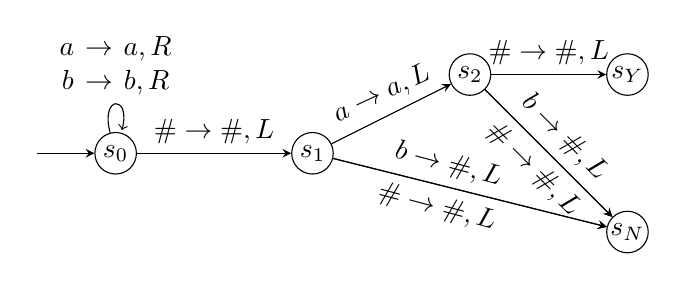
\begin{tikzpicture}
        \node[circle, draw=black, fill=white, inner sep=0pt, minimum size=15pt] (s0) at (-0.5, 0) {$s_0$};
        \node[circle, draw=black, fill=white, inner sep=0pt, minimum size=15pt] (s1) at (2, 0) {$s_1$};
        \node[circle, draw=black, fill=white, inner sep=0pt, minimum size=15pt] (s2) at (4, 1) {$s_2$};
        \node[circle, draw=black, fill=white, inner sep=0pt, minimum size=15pt] (sY) at (6, 1) {$s_Y$};
        \node[circle, draw=black, fill=white, inner sep=0pt, minimum size=15pt] (sN) at (6, -1) {$s_N$};
        
        \draw[-stealth] (-1.5, 0) -- (s0);
        \draw[-stealth] (s0) edge[loop above] node[align=center, text width=2cm] {$a \to a, R$ $b \to b, R$} (s0);
        \draw[-stealth] (s0) -- node[above] {$\# \to \#, L$} (s1);

        \draw[-stealth] (s1) -- node[above, rotate=25] {$a \to a, L$} (s2);
        \draw[-stealth] (s1) -- node[below, rotate=-15, pos=0.4] {$\# \to \#, L$} (sN);
        \draw[-stealth] (s1) -- node[above, rotate=-15, pos=0.4] {$b \to \#, L$} (sN);

        \draw[-stealth] (s2) -- node[above] {$\# \to \#, L$} (sY);

        \draw[-stealth] (s2) -- node[above, rotate=-45] {$b \to \#, L$} (sN);
        \draw[-stealth] (s2) -- node[below, rotate=-45] {$\# \to \#, L$} (sN);
    \end{tikzpicture}
    \caption{The TM corresponding to the program above. The state $s_0$ corresponds to the module \texttt{moveToEnd}; the state $s_1$ corresponds to the module \texttt{checkAFirst}; and the state $s_2$ corresponds to the module \texttt{checkASecond}.}
\end{figure}
    
\begin{appendices}

% Use separate appendix chapters for groups of ancillary material that support your dissertation. 
% Typical inclusions in the appendices are:

% \begin{itemize}
% \item
%   Copies of ethics approvals (you must include these if you needed to get them)
% \item
%   Copies of questionnaires etc. used to gather data from subjects. Don't include
%   voluminous data logs; instead submit these electronically alongside your source code.
% \item
%   Extensive tables or figures that are too bulky to fit in the main body of
%   the report, particularly ones that are repetitive and summarised in the body.
% \item Outline of the source code (e.g. directory structure), 
%     or other architecture documentation like class diagrams.
% \item User manuals, and any guides to starting/running the software. 
% Your equivalent of \texttt{readme.md} should be included.

% \end{itemize}

% \textbf{Don't include your source code in the appendices}. It will be
% submitted separately.



\chapter{Proofs of the Theorems}
\setcounter{theorem}{0}

\begin{theorem} \label{thm:complete_TM}
    Let $P$ be a valid TML program. Then, $P$ and its completion $P^+$ execute on every valid tape $T$ in the same way. That is,
    \begin{itemize}
        \item for every valid index $n$, if we have tape $T_n$, tapehead index $i_n$ and module $m_n$ with executing block $b_n$ for the TM program $P$, and we have tape $S_n$, tapehead index $j_n$ and module $t_n$, then $T_n = S_n$, $i_n = j_n$, and $t_n$ is the corresponding complete module block of $b_n$;
        \item $P$ terminates execution on $T$ if and only if $P^+$ terminates execution on $T$, with the same final status (\texttt{accept} or \texttt{reject}).
    \end{itemize}
\end{theorem}
\begin{proof}
    We prove this by induction on the execution step (of the tape). 
    \begin{itemize}
        \item At the start, we have the same tape $T$ for both $P$ and $P^+$, with tapehead index 0. Moreover, the corresponding (completed) module of the first block in the first module of $P$ is the first module of $P$. So, the result is true if $n = 0$. 
        \item Now, assume that the result is true for some integer $n$, where the block $b_n$ in the TML program $P$ does not end with a terminating \textit{flow} command. Let $\sigma_n$ be the letter at index $i_n = j_n$ on the tape $S_n = T_n$.
        \begin{itemize}
            \item If the \textit{changeto} command is missing in $b_n$ for $\sigma_n$, then the next tape $T_{n+1} = T_n$. In the complete module $m_n$, the case for $\sigma_n$ will have the command \texttt{changeto} $\sigma_n$. So, the next tape is given by:
            \[S_{n+1}(x) = \begin{cases}
                S_n(x) & x \neq j_n \\
                \sigma_n & \text{otherwise}
            \end{cases}.\]
            Therefore, we have $S_{n+1} = S_n$ as well. So, $T_{n+1} = S_{n+1}$. Otherwise, we have the same \textit{changeto} command in the two blocks, in which case $T_{n+1} = S_{n+1}$ as well.
            
            \item If the \textit{move} command is missing in $b_n$ for $\sigma_n$, then the next tapehead index $i_{n+1} = i_n - 1$. In the complete module $m_n$, the case for $\sigma_n$ will have the command \texttt{move left}, so we also have $j_{n+1} = j_n - 1$. Applying the inductive hypothesis, we have $i_{n+1} = j_{n+1}$. Otherwise, we have the same \textit{move} command, meaning that $i_{n+1} = j_{n+1}$ as well.
            
            \item We now consider the next block $b_{n+1}$:
            \begin{itemize}
                \item If the block $b_n$ is a \textit{switch} block with a \textit{while} case for $\sigma_n$, then this is still true in the module $m_n$. So, the next block to be executed in $P$ is $b_n$, and the next module to be executed in $P^+$ is $m_n$. In that case, the corresponding module of the block $b_{n+1} = b_n$ is still $m_{n+1} = m_n$.
    
                \item Instead, if the block $b_n$ has no \textit{flow} command for $\sigma_n$, and is not the last block, then the next block to execute is the block just below $b_n$, referred as $b_{n+1}$. By the definition of $P^+$, we find that the case block in the module $m_n$ has a \textit{goto} command, going to the module $m_{n+1}$ which corresponds to the block $b_{n+1}$. 
            
                \item Now, if the \textit{flow} command is missing for $\sigma_n$ and this is the last block, then execution is terminated with the status \texttt{reject} for the program $P$. In that case, the case for $\sigma_n$ in the module $m_n$ has the \texttt{reject} command present, so the same happens for $P^+$ as well. 
            
                \item Otherwise, both $P$ and $P^+$ have the same flow command, meaning that there is either correspondence between the next module to be executed, or both the program terminate with the same status. 
            \end{itemize}
        \end{itemize}
    \end{itemize}
    In that case, $P$ and $P^+$ execute on $T$ the same way by induction.
\end{proof}

\begin{theorem} \label{thm:TM_to_TMP}
    Let $M$ be a TM, and let $P$ be the corresponding program for $M$. Then, $M$ and $P$ execute on every valid tape $T$ in the same way. That is, 
    \begin{itemize}
        \item for every valid index $n$, if we have tape $T_n$, tapehead index $i_n$ and module $m_n$ for the TM program $P$, and we have tape $S_n$, tapehead index $j_n$ and state $q_n$ for the TM $M$, then $T_n = S_n$, $i_n = j_n$ and $m_n$ is the corresponding module for $q_n$;
        \item $M$ terminates execution on $T$ if and only if $P$ terminates execution on $T$, with the same final status (\texttt{accept} or \texttt{reject}).
    \end{itemize}
\end{theorem}
\begin{proof}
    We prove this by induction on the execution step. 
    \begin{itemize}
        \item At the start, we have the same tape $T$ for both $M$ and $P$, with tapehead index $0$. Moreover, the first module in $P$ corresponds to the initial state $q_0$. So, the result is true if $n = 0$.
        
        \item Now, assume that the result is true for some integer $n$, where the TM state $q_n$ is not \texttt{accept} or \texttt{reject}. In that case, $T_n = S_n$, $i_n = j_n$ and $m_n$ is the corresponding module for $q_n$. Let $\sigma_n$ be the letter at index $i_n = j_n$ on the tape $T_n = S_n$. Denote $q(q_n, \sigma_n) = (q_{n+1}, \sigma_{n+1}, \texttt{dir})$. In that case,
        \[T_{n+1}(x) = \begin{cases}
            T_n(x) & x \neq i_n \\
            \sigma_{n+1} & \text{otherwise},
        \end{cases} \qquad i_{n+1} = \begin{cases}
            i_n - 1 & \texttt{dir} = \texttt{left} \\
            i_n + 1 & \texttt{dir} = \texttt{right},
        \end{cases}\]
        and the next state is $q_{n+1}$. 
        
        \begin{itemize}
            \item We know that the module $m_n$ in TM program $P$ corresponds to the state $q_n$, so it has a \texttt{changeto} $\sigma_{n+1}$ command for the case $\sigma_n$. In the case, the next tape for $P$ is:
            \[S_{n+1}(x) = \begin{cases}
                S_n(x) & x \neq i_n \\
                \sigma_{n+1} & \text{otherwise}.
            \end{cases}\]
            So, $T_{n+1} = S_{n+1}$. 
            
            \item Similarly, the case also contains a \texttt{move dir} command. This implies that the next tapehead index for $P$ is:
            \[j_{n+1} = \begin{cases}
                j_n - 1 & \texttt{dir} = \texttt{left} \\
                j_n + 1 & \texttt{dir} = \texttt{right}.
            \end{cases}\]
            Hence, $i_{n+1} = j_{n+1}$. 
        
            \item Next, we consider the value of $q_{n+1}$:
            \begin{itemize}
                \item If $q_{n+1} = q_n$, then the case block is a \textit{while} block, and vice versa. So, the next module to be executed is $m_n$. In that case, $m_{n+1}$ still corresponds to $q_{n+1}$.
                \item Otherwise, we have an \textit{if} block. 
                \begin{itemize}
                    \item In particular, if $q_{n+1}$ is the \texttt{accept} state, then the case for $\sigma_n$ contains the \textit{flow} command \texttt{accept}, and vice versa. In that case, execution terminates with the same final status of \texttt{accept}. The same is true for \texttt{reject}. 
                    \item Otherwise, the module contains the command \texttt{goto} $m_{n+1}$, where $m_{n+1}$ is the corresponding module for $q_{n+1}$.
                \end{itemize}
            \end{itemize}
        \end{itemize}
        % Therefore, if the result holds for $n$, it holds for $n+1$. So, the result follows from induction.
    \end{itemize}
    In that case, $P$ and $M$ execute on $T$ the same way by induction.
\end{proof}

\begin{theorem}
    Let $P$ be a complete TM program, and let $M$ be the corresponding TM for $P$. Then, $P$ and $M$ execute on every valid tape $T$ in the same way. That is,
    \begin{itemize}
        \item for every valid index $n$, if we have tape $T_n$, tapehead index $i_n$ and module $m_n$ for TM program $P$, and we have tape $S_n$, tapehead index $j_n$ and state $q_n$ for the TM $M$, then $T_n = S_n$, $i_n = j_n$ and $q_n$ is the corresponding state for $m_n$;
        \item $P$ terminates execution on $T$ if and only if $M$ terminates execution on $T$, with the same final status (\texttt{accept} or \texttt{reject}).
    \end{itemize}
\end{theorem}
\begin{proof}
    We prove this as well by induction on the execution step of the tape. 
    \begin{itemize}
        \item At the start, we have the same tape $T$ for both $P$ and $M$, with tapehead index $0$. Moreover, the initial state $q_0$ in $M$ corresponds to the first module in $P$. So, the result is true if $n = 0$. 
        
        \item Now, assume that the result is true for some integer $n$, which is not the terminating step in execution. In that case, $S_n = T_n$, $j_n = i_n$ and $q_n$ is the corresponding state for $m_n$. Let $\sigma_n$ be the letter at index $j_n = i_n$ on the tape $S_n = T_n$. We now consider the single switch block in $m_n$:
        \begin{itemize}
            \item If the block in $m_n$ corresponding to $\sigma_n$ is a \textit{while} block, then we know that its body is partially complete, and so is composed of the following commands:
            \begin{itemize}
                \item \texttt{changeto} $\sigma_{n+1}$
                \item \texttt{move dir}
            \end{itemize}
            So, we have $\delta(q_n, \sigma_n) = (q_n, \sigma_{n+1}, \texttt{dir})$. Using the same argument as in Theorem \ref{thm:TM_to_TMP}, we find that $T_{n+1} = S_{n+1}$ and $i_{n+1} = j_{n+1}$. Also, $q_{n+1} = q_n$ is the corresponding state for $m_{n+1} = m_n$. 
            
            \item Otherwise, we have an \textit{if} command. In this case, the case body is complete, and so composed of the following commands:
            \begin{itemize}
                \item \texttt{changeto} $\sigma_{n+1}$
                \item \texttt{move dir}
                \item \texttt{accept}, \texttt{reject} or \texttt{goto} $m_{n+1}$.
            \end{itemize}
            So, we have $\delta(q_n, \sigma_n) = (q_{n+1}, \sigma_{n+1}, \texttt{dir})$, where $q_{n+1}$ is the corresponding state to the \textit{flow} command present. Here too, we have $T_{n+1} = S_{n+1}$ and $i_{n+1} = j_{n+1}$ by construction. 
        \end{itemize}
        Now, we consider the flow command:
        \begin{itemize}
            \item If we have an \texttt{accept} command in the body, then $q_{n+1}$ is the accepting state, and vice versa. So, we terminate execution with the final status of \texttt{accept}. The same is true for \texttt{reject}. 
            \item Otherwise, the state $q_{n+1}$ is the corresponding state to the module $m_{n+1}$.
        \end{itemize}
        In all cases, there is a correspondence between the state for $m_{n+1}$ and $q_{n+1}$.   
    \end{itemize}
    So, the result follows from induction.
\end{proof}



\end{appendices}

\end{appendices}

%==================================================================================================================================
%   BIBLIOGRAPHY   

% The bibliography style is agsm (Harvard)
% The bibliography always appears last, after the appendices.

\bibliographystyle{agsm}

% Force the bibliography not to be numbered
\renewcommand{\thechapter}{0} 
\bibliography{l4proj}

\end{document}
